% The covering projection R -> S^1 as a helix projected down onto the circle.
% Source: book/tex/topology/cover-project.tex (§ Even coverings and covering projections).
\documentclass[border=2mm]{standalone}
\usepackage{tikz}
\usepackage{amssymb}
\usetikzlibrary{arrows.meta}
\begin{document}
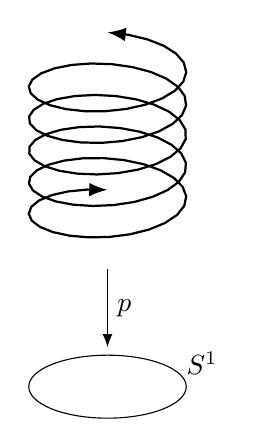
\begin{tikzpicture}[scale=1]
  % helix: several turns, foreshortened vertically
  \draw[{Latex}-{Latex},thick]
    plot[domain=90:1890,samples=120,variable=\a]
      ({cos(\a)},{0.4*sin(\a)+\a/900});
  % projection arrow
  \draw[-{Latex}] (0,-0.5) -- (0,-1.5) node[midway,right] {$p$};
  % S^1
  \draw (0,-2) ellipse (1 and 0.4);
  \node at (1.2,-1.7) {$S^1$};
\end{tikzpicture}
\end{document}
